% Einführing in die FEM mit Hilfe von Grossman S.175
Im Vorherigen Kapitel haben wir das Ritz-Galerkin Verfahren kennengelernt. Der Kernaspekt dieser konformer Approximation war eine diskretisierung des Raumes und mit einhergehend global einheitlich definierte Funktionen. Nun öffnen wir die letzt genannte Einschränkung und fordern nur noch stückweise definierte Funktionen, in der Regel Polynome. Wo genau eine Funktion definiert ist, hängt von unsererer Gebietszerlegung ab.
Das heißt für die Finite Elemente Methode (FEM) ist es zu erst notwendig das Grundgebiet in geometrisch einfache Teilgebiete $\Omega_h = \{\Omega_k \}_{k=1 \dots N}$ z.B. Dreiecke und Rechtecke bei Problemen in der Ebene oder Tetraeder und Quader bei Problemen im dreidimensionalen Raum.
Dann folgt eine Definition von Ansatz- und Testfunktionen über Teilgebieten. Da wir zwischen den Teilgebieten eine Stetigkeit fordern, definiert man Übergangsbedigungen die dann die Sicherung der Stetigkeit global sichert. (Grossmann Seite 175).
Die Stetigkeit wird gefordert damit wir $V_n \subset V$ bekommen, da beispielsweise gelten kann $V \subset H^1 (\Omega)$. 

\begin{Bemerkung} Natürliche Voraussetzungen an Zerlegung (Grossman S.176) \\
Die Voraussetzungen an die Zerlegung {\calligra{Z}}=$\{ \Omega_j \}_{j=1}^{m}$ sind 
\begin{enumerate}
\item \begin{equation*}
\bar{\Omega} = \bigcup\limits_{j=1}^{m} \bar{\Omega_j} 
\end{equation*}
\item \begin{equation*}
 int \Omega_i \cap int \Omega_j = \emptyset \text{ , falls } i \neq j.
\end{equation*}
\end{enumerate}
\end{Bemerkung}


\begin{Beispiel} $\Omega = [a,b]$ (Grossmann S.184) \\
Wir definieren Gitterpunkte $\{x_i\}_{i=0}^{N}$ über $\bar\Omega$  beschrieben wie folgt:
\begin{equation*}
a = x_0 < x_1 < x_2 < \dots < x_{N-1} < x_N = b
\end{equation*}
und eine Zerlegung  {\calligra{Z}}=$\{ \Omega_j \}_{j=1}^{m}$ mit $\Omega_i := (x_{i-1},x_i)$ $i=1,\dots,N$. 
\end{Beispiel}
Ferner sei $h_i := x_i - x_{i-1}, i=1,\dots,N$. Wir wählen lineare Ansatzfunktionen damit gilt $V_h=lin\{\phi_i\}_{i=0}^{N}$ wobei die Ansatzfunktionen definiert sind durch
\begin{equation}
\begin{aligned}
\phi_i(x) &= 
\begin{cases}
\dfrac{1}{h_i}(x-x_{i-1}) \text{, für } x \in \Omega_i \\
\dfrac{1}{h_{i+1}}(x_{i+1}-x) \text{ für } x \in \Omega_{i+1}  \\
0 \text{, sonst }
\end{cases}
\end{aligned}
\end{equation}

Es gilt nach Konstruktion $\phi \in C(\bar{\Omega})$ sowie $\phi_{i} \Big|_{\Omega_{j}} \in C^{1}(\bar{\Omega_{j}})$, somit hat man insgesamt $\phi_i \in H^{1}(\Omega)$.
Die folgende Abbildung stellt die Graphen von Ansatzfunktionen $\phi_i$ dar.

\begin{figure}[ht]
	\centering
  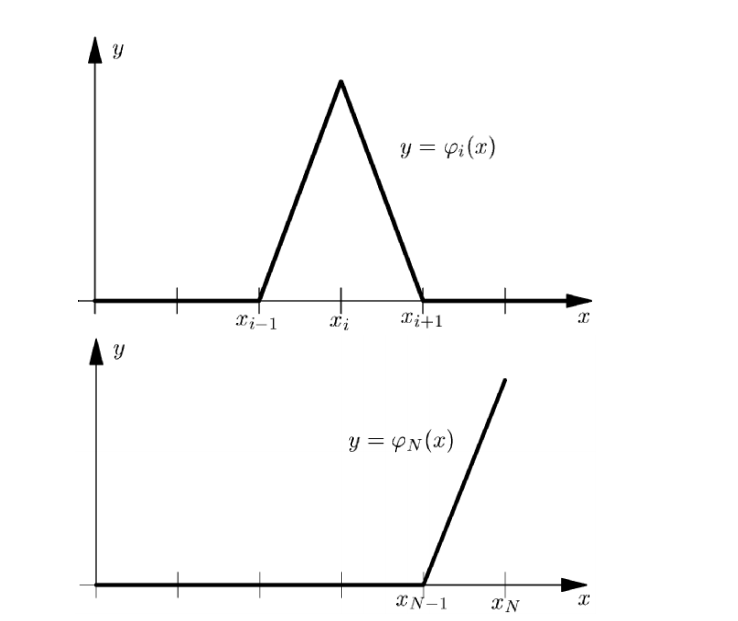
\includegraphics[width=0.7\textwidth]{hatfunction.png}
	\caption{Ansatzfunktionen $\phi_i$}
	\label{fig:hat}
\end{figure}

Es gilt demnach $\phi_i (x_k) = \delta_{ik}, i,k =0,1,\dots,N$.
